\documentclass[xcolor=pdftex,dvipsnames,table,mathserif,aspectratio=169]{beamer}
\usetheme{default}
\usetheme{metropolis}
\usepackage{mathtools}
\setbeamersize{text margin left=.3in,text margin right=.3in}

\DeclarePairedDelimiter\abs{\lvert}{\rvert}%
\DeclarePairedDelimiter\norm{\lVert}{\rVert}%

\usepackage[english]{babel}
\usepackage{pgf,pgfarrows,pgfnodes,pgfautomata,pgfheaps}
\usepackage{amsmath,amssymb,setspace,centernot}
\usepackage[latin1]{inputenc}
\usepackage{pgf,tikz}
\usepackage[T1]{fontenc}
\usepackage{relsize}
\usepackage{pdfpages}
\usepackage[absolute,overlay]{textpos}


\newenvironment{reference}[2]{%
  \begin{textblock*}{\textwidth}(#1,#2)
      \footnotesize\it\bgroup\color{red!50!black}}{\egroup\end{textblock*}}

\DeclareMathSizes{10}{10}{6}{6}

\begin{document}
\title{Multinomial Discrete Choice: IIA Logit}
\author{Chris Conlon}
\institute{Grad IO}
\date{\today}

\frame{\titlepage}


\begin{frame}
\frametitle{Motivation}
Most decisions agents make are not necessarily binary:
\begin{itemize}
\item Choosing a level of schooling (or a major).
\item Choosing an occupation.
\item Choosing a partner.
\item Choosing where to live.
\item Choosing a brand of (yogurt, laundry detergent, orange juice, cars, etc.).
 \end{itemize}
\end{frame}

\begin{frame}
\frametitle{Nonparametric Setup}
We consider a \alert{multinomial discrete choice}:
\begin{itemize}
\item in period $t$
\item with $\mathcal{J}_t$ alternatives.
\item subscript individual agents by $i$.
\item agents choose $j \in J_t$ with probability $S_{ijt}$.
\item Agent $i$ receives utility $U_{ij}$ for choosing $j$.
\item Choice is exhaustive and mutually exclusive.
 \end{itemize}\pause
Consider the simple example $(t=1)$:
\begin{eqnarray*}
s_{ij} = Prob( U_{ij} > U_{ik} \quad \forall j \neq k)
\end{eqnarray*}
\end{frame}

\begin{frame}
\frametitle{Nonparametric Setup}
Now consider separating the utility into the \alert{observed} $V_{ij}$ and \alert{unobserved} components $\varepsilon_{ij}$.
\begin{eqnarray*}
s_{ij} &=& Prob( U_{ij} > U_{ik} \quad \forall j \neq k)\\
 &=& Prob( V_{ij} + \varepsilon_{ij} > V_{ik} + \varepsilon_{ik} \quad \forall j \neq k)\\
 &=& Prob( \varepsilon_{ij}-\varepsilon_{ik} > V_{ik} - V_{ij} \quad \forall j \neq k)
\end{eqnarray*}
\pause
It is helpful to define $f(\varepsilon_{i})$ as the $J$ vector of individual $i$'s unobserved utility.
\begin{eqnarray*}
s_{ij} &=& Prob( \varepsilon_{ij}-\varepsilon_{ik} > V_{ik} - V_{ij} \quad \forall j \neq k)\\
&=& \int I( \varepsilon_{ij}-\varepsilon_{ik} > V_{ik} - V_{ij} ) f( \varepsilon_i) \partial \varepsilon_i \\
\end{eqnarray*}
\end{frame}

\begin{frame}
\frametitle{Nonparametric Setup}
In order to compute the choice probabilities, we must perform a $J$ dimensional integral over $f(\varepsilon_i)$.
\begin{eqnarray*}
s_{ij} &=&  \int I( \varepsilon_{ij}-\varepsilon_{ik} > V_{ik} - V_{ij} ) f( \varepsilon_i) \partial \varepsilon_i
\end{eqnarray*}
There are some choices that make our life easier
\begin{itemize}
\item Multivariate normal: $\varepsilon_i  \sim N(0,\Omega)$. $\longrightarrow$ \alert{ multinomial probit}.
\item Gumbel/Type 1 EV: $f(\varepsilon_i) = e^{-\varepsilon_{ij}}  e^{-e^{-\varepsilon_{ij}}}  $ and $F(\varepsilon_i) = 1- e^{-e^{-\varepsilon_{ij}}}$ $\longrightarrow$ \alert{multinomial logit}
\item There are also heteroskedastic variants of the Type I EV/ Logit framework.
\end{itemize}
\end{frame}

\begin{frame}
\frametitle{Errors}
Allowing for full support $(-\infty, \infty)$ errors provide two key features:
\begin{itemize}
\item Smoothness: $s_{ij}$ is everywhere continuously differentiable in $V_{ij}$.
\item Bound $s_{ij} \in (0,1)$ so that we can rationalize any observed pattern in the data.
\begin{itemize}
\item Caveat: zero and one (interpretation).
\end{itemize}
\item What does $\varepsilon_{ij}$ really mean? (unobserved utility, idiosyncratic tastes, etc.)
\end{itemize}
\end{frame}

\begin{frame}
\frametitle{Basic Identification}
\small
\begin{itemize}
\item Only differences in utility matter: $Prob( \varepsilon_{ij}-\varepsilon_{ik} > V_{ik} - V_{ij} \quad \forall j \neq k)$
\item Adding constants is irrelevant: if $U_{ij} > U_{ik}$ then $U_{ij} + a > U_{ik} + a$.
\item Only differences in alternative specific constants can be identified
\begin{eqnarray*}
U_b &=& X_b \beta + k_b  + \varepsilon_b\\
U_c &=& X_c \beta + k_c  + \varepsilon_c
\end{eqnarray*}
only $d = k_b - k_c$ is identified.
\item This means that we can only include $J-1$ such $k$'s and need to normalize one to zero. (Much like fixed effects).
\item We cannot have individual specific factors that enter the utility of all options such as income $\theta Y_i$. We can allow for interactions between individual and choice characteristics $\theta p_{j}/ Y_i$.
\end{itemize}
\end{frame}

\begin{frame}
\frametitle{Basic Identification: Location}
\begin{itemize}
\item Technically we can't really fully specify $f(\varepsilon_i)$ since we can always re-normalize: $\widetilde{\varepsilon_{ijk}} = \varepsilon_{ij} - \varepsilon_{ik}$ and write $g(\widetilde{\varepsilon_{ik}})$. Thus any $g(\widetilde{\varepsilon_{ik}})$ is consistent with infinitely many $f(\varepsilon_i)$.
\item Logit pins down $f(\varepsilon_i)$ sufficiently with parametric restrictions.
\item Probit does not. We must generally normalize one dimension of $f(\varepsilon_i)$ in the probit model. Usually a diagonal term of $\Omega$ so that $\omega_{11} =1$ for example. (Actually we need to do more!).
\end{itemize}
\end{frame}



\begin{frame}
\frametitle{Basic Identification: Scale}
\begin{itemize}
\item Consider: $U_{ij}^0 = V_{ij} + \varepsilon_{ij}$ and  $U_{ij}^1 = \lambda V_{ij} + \lambda \varepsilon_{ij}$ with $\lambda > 0$. Multiplying by constant $\lambda$ factor doesn't change any statements about $U_{ij} > U_{ik}$.
\item We normalize this by fixing the variance of $\varepsilon_{ij}$ since $Var(\lambda \varepsilon_{ij} ) = \sigma_e^2 \lambda^2$.
\item Normalizing this variance normalizes the scale of utility.
\item For the logit case the variance is normalized to $\pi^2/6$. (this emerges as a constant of integration to guarantee a proper density).
\end{itemize}
\end{frame}



\begin{frame}
\frametitle{Observed Heteroskedasticity}
Consider the case where $Var(\varepsilon_{ij}^B) = \sigma^2$ and   $Var(\varepsilon_{ij}^C) =  k^2 \sigma^2$ :
\begin{itemize}
\item We can estimate
\begin{eqnarray*}
U_{ij} &=& x_j \beta + \varepsilon_{ij}^B\\
U_{ij} &=& x_j \beta + \varepsilon_{ij}^C
\end{eqnarray*}
becomes:
\begin{eqnarray*}
U_{ij} &=& x_j \beta + \varepsilon_{ij}\\
U_{ij} &=& x_j \beta/k+ \varepsilon_{ij}
\end{eqnarray*}
\item Some interpret this as saying that in segment $C$ the unobserved factors are $\hat{k}$ times larger.
\end{itemize}
\end{frame}

\begin{frame}
\frametitle{Deeper Identification Results}
Different ways to look at identification
\begin{itemize}
\item Are we interested in non-parametric identification of $V_{ij}$, specifying $f(\varepsilon_i)$?
\item Or are we interested in non-parametric identification of $U_{ij}$. (Generally hard).
\begin{itemize}
\item Generally we require a large support (special-regressor) or ``completeness'' condition.
\item Lewbel (2000) does random utility with additively separable but nonparametric error.\item Berry and Haile (2015) with non-separable error (and endogeneity).
\end{itemize}
\end{itemize}
\end{frame}


\begin{frame}
\frametitle{Multinomial Logit}
\begin{itemize}
\item Multinomial Logit (Gumbel/Type I EV) has closed form choice probabilities
\begin{eqnarray*}
s_{ij} = \frac{e^{V_{ij}}}{\sum_k e^{V_{ik}}}
\end{eqnarray*}
\item Often we approximate $V_{ij} \approx  X_{ik} \beta$ with something linear in parameters.
\end{itemize}
\end{frame}


\begin{frame}
\frametitle{Logit Inclusive Value}
 Expected maximum also has closed form:
\begin{eqnarray*}
E[\max_j U_{ij}] = \log \left(\sum_j \exp[V_{ij}] \right) + C
\end{eqnarray*}
Logit Inclusive Value is helpful for several reasons
\begin{itemize}
\item Expected utility of best option (without knowledge of $\varepsilon_i$) does not depend on $\epsilon_{ij}$.
\item This is a globally concave function in $V_{ij}$ (more on that later).
\item Allows simple computation of $\Delta CS$ for consumer welfare (but not $CS$ itself).
\end{itemize}
\end{frame}

\begin{frame}
\frametitle{Multinomial Logit}
Multinomial Logit goes by a lot of names in various literatures
\begin{itemize}
\item The problem of multiple choice is often called \alert{multiclass classification} or \alert{softmax regression} in other literatures.
\item In general these models assume you have individual level data
\end{itemize}
\end{frame}

\begin{frame}
\frametitle{Alternative Interpretation}
Statistics/Computer Science offer an alternative interpretation
\begin{itemize}
\item Sometimes this is called \alert{softmax} regression.
\item Think of this as a continuous/concave approximation to the maximum.
\item Consider $\max\{x,y\}$ vs $\log(\exp(x) + \exp(y))$. The $\exp$ exaggerates the differences between $x$ and $y$ so that the larger term dominates.
\item We can accomplish this by rescaling $k$:  $\log(\exp(kx) + \exp(ky))/k$ as $k$ becomes large the derivatives become infinite and this approximates the ``hard'' maximum.
\item $g(1, 2) = 2.31$, but $g(10, 20) = 20.00004$.
\end{itemize}
\end{frame}

\begin{frame}{Alternative Interpretation}
\begin{figure}[htbp]
\begin{center}
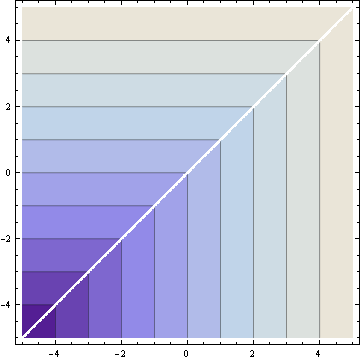
\includegraphics[width=2in]{./resources/hardmax.png}
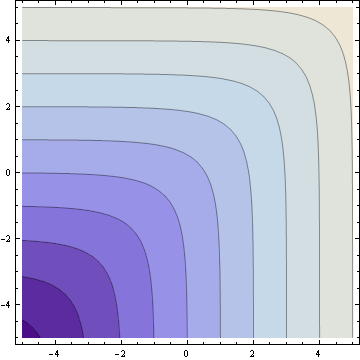
\includegraphics[width=2in]{./resources/softmax.png}
\end{center}
\end{figure}
\end{frame}

\begin{frame}
\frametitle{Multinomial Logit: Identification}
What is actually identified here?
\begin{itemize}
\item Helpful to look at the ratio of two choice probabilities
\begin{align*}
\frac{s_{ij}(\theta)}{s_{ik}(\theta)}  = \frac{e^{V_ij}}{e^{V_{ik}}} = e^{V_{ij} - V_{ik}}
\end{align*}
\item We only identify the \alert{difference in indirect utilities} not the levels.
\item The ratio of choice probabilities for $j$ and $k$ depends only on $j$ and $k$ and not on any alternative $l$, this is known as \alert{independence of irrelevant alternatives}.
\item For some (Luce (1959)) IIA was an attractive property for axiomatizing choice. (A feature or a bug?)
\item In fact the logit was derived in the search for a statistical model that satsified various axioms.
\end{itemize}
\end{frame}

\begin{frame}
\frametitle{Multinomial Logit: Identification}
As another idea suppose we add a constant $C$ to each $\beta_j$.
\begin{eqnarray*}
s_{ij} = \frac{\exp[\mathbf{x_i} (\beta_j+C) ]}{\sum_k \exp[\mathbf{x_i} (\beta_k+C) ]} =  \frac{\exp[\mathbf{x_i} C] \exp[\mathbf{x_i} \beta_j ]}{\exp[\mathbf{x_i} C] \sum_k \exp[\mathbf{x_i} \beta_k ]}
\end{eqnarray*}
This has no effect.  That means we need to fix a normalization $C$.\\
 The most convenient is generally that $C = - \beta_K$.
\begin{itemize}
\item We normalize one of the choices to provide a utility of zero.
\item We actually already made another normalization. Does anyone know which?
\end{itemize}
\end{frame}


\begin{frame}
\frametitle{Multinomial Logit: Identification}
The most sensible normalization in demand settings is to allow for an \alert{outside option} which produces no utility in expectation so that $e^{V_{i0}} = e^{0}=1$:
\begin{eqnarray*}
s_{ij} = \frac{e^{V_{ij} }}{1+\sum_k e^{V_{ik} }}
\end{eqnarray*}
\begin{itemize}
\item Hopefully the choice of outside option is well defined: not buying a yogurt, buying some other used car, etc.
\item Now this resembles the binomial logit model more closely.
\end{itemize}
\end{frame}


\begin{frame}{Back to Scale of Utility}
\begin{itemize}
\item Consider $U_{ij}^{*} = V_{ij} + \varepsilon_{ij}^{*}$ with $Var(\varepsilon^{*}) = \sigma^2 \pi^2/6$.
\item Without changing behavior we can divide by $\sigma$ so that $U_{ij} = V_{ij}/\sigma + \varepsilon_{ij}$ and $Var(\varepsilon^{*}/\sigma)=Var(\varepsilon) = \pi^2/6$
\begin{eqnarray*}
s_{ij} = \frac{e^{V_{ij}/\sigma}}{\sum_k e^{V_{ik}/\sigma}} \approx \frac{e^{\beta^{*}/\sigma \cdot x_{ij}}}{\sum_k e^{\beta^{*}/\sigma \cdot x_{ik}}}
\end{eqnarray*}
\item Every coefficient $\beta$ is rescaled by $\sigma$. This implies that only the ratio $\beta^{*}/\sigma$ is identified.
\item Coefficients are relative to variance of unobserved factors. More unobserved variance $\longrightarrow$ smaller $\beta$.
\item Ratio $\beta_1/\beta_2$ is invariant to the scale parameter $\sigma$. (\alert{marginal rate of substitution}).
\end{itemize}
\end{frame}

%
%\begin{frame}{Taste Variation}
%\begin{eqnarray*}
%\frac{s_{ij}}{s_{ik}} = \frac{e^{V_{ij}}}{\sum_{k'} e^{V_{ik'}}} / \frac{e^{V_{ik}}}{\sum_{k'} e^{V_{ik'}}} = \frac{e^{V_{ij}}}{e^{V_{ik}}} = \exp[V_{ij} - V_{ik}].
%\end{eqnarray*}
%\begin{itemize}
%\item The ratio of choice probabilities for $j$ and $k$ depends only on $j$ and $k$ and not on any alternative $l$, this is known as \alert{independence of irrelevant alternatives}.
%\item For some (Luce (1959)) IIA was an attractive property for axiomatizing choice.
%\item In fact the logit was derived in the search for a statistical model that satsified various axioms.
%\end{itemize}
%\end{frame}

\begin{frame}{IIA Property}
The well known critique:
\begin{itemize}
\item You can choose to go to work on a car $c$ or blue bus $bb$. $S_{c} = S_{bb} = \frac{1}{2}$ so that $\frac{S_c}{S_{bb}} = 1$.
\item Now we introduce a red bus $rb$ that is identical to $bb$. Then $\frac{S_{rb}}{S_{bb}} = 1$ and $S_{c} = S_{bb}= S_{rb} = \frac{1}{3}$ as the logit model predicts.
\item In reality we don't expect painting a bus red would change the number of individuals who drive a car so we would anticipate $S_{c} = \frac{1}{2}$ and $S_{bb} = S_{rb} = \frac{1}{4}$.
\item We may not encounter too many cases where $\rho_{\varepsilon_{ik},\varepsilon_{ij}} \approx 1$, but we have many cases where this $\rho_{\varepsilon_{ik},\varepsilon_{ij}} \neq 0$
\item What we need is the ratio of probabilities to change when we introduce a third option!
\end{itemize}
\end{frame}

\begin{frame}{IIA Property}
\begin{itemize}
\item IIA implies that we can obtain consistent estimates for $\beta$ on any subset of alternatives.
\item This means instead of using all $\mathcal{J}$ alternatives in the choice set, we could estimate on some subset $\mathcal{S} \subset \mathcal{J}$.
\item This used to be a way to reduce the computational burden of estimation (not clear this is an issue in 21st century).
\item Sometimes we have \alert{choice based samples} where we oversample people who choose a particular alternative. Manski and Lerman (1977) show we can get consistent estimates for all but the ASC. This requires knowledge of the difference between the true rate $A_j$ and the choice-based sample rate $\mathcal{S}_j$.
\item Hausman proposes a specification test of the logit model: estimate on the full dataset to get $\hat{\beta}$, construct a smaller subsample $\mathcal{S}^k \subset \mathcal{J}$ and $\hat{\beta^k}$ for one or more subsets $k$. If $|\hat{\beta}^k - \hat{\beta}|$ is small enough.
\end{itemize}
\end{frame}

\begin{frame}{IIA Property}
\small
For the linear $V_{ij}$ case we have that $\frac{\partial V_{ij}}{\partial z_{ij}}=  \beta_z$.
\begin{eqnarray*}
\frac{\partial s_{ij}}{\partial z_{ij}} = s_{ij}(1- s_{ij}) \frac{\partial V_{ij}}{\partial z_{ij}}
\end{eqnarray*}
\begin{eqnarray*}
\text{ And Elasticity: }\quad  \frac{ \partial \log s_{ij}}{ \partial \log z_{ij}} = s_{ij}(1- s_{ij}) \frac{\partial V_{ij}}{\partial z_{ij}} \frac{z_{ij}}{s_{ij}} = (1- s_{ij}) z_{ij} \frac{\partial V_{ij}}{\partial z_{ij}}
\end{eqnarray*}
\begin{eqnarray*}
\text{ With cross effects: }\ \frac{\partial s_{ij}}{\partial z_{ik}} = -s_{ij} s_{ik} \frac{\partial V_{ik}}{\partial z_{ik}}
\end{eqnarray*}
\begin{eqnarray*}
\text{ and elasticity : }\quad \frac{ \partial \log s_{ij}}{ \partial \log z_{ik}} = -s_{ik} z_{ik} \frac{\partial V_{ik}}{\partial z_{ik}}
\end{eqnarray*}
\end{frame}

\begin{frame}
\frametitle{Own and Cross Elasticity}
An important output from a demand system are elasticities
\begin{itemize}
\item This implies that $ \eta_{jj} = \frac{\partial s_{ij}}{\partial p_j} \frac{p_j}{s_{ij}}  = \beta_p \cdot p_j \cdot (1-s_{ij})$.
\item The price elasticity is increasing in own price! (Why is this a bad idea?)
\item Also mechanical relationship between elasticity and \alert{share} so that popular products necessarily have higher markups (holding fixed prices).
\end{itemize}
\end{frame}



\begin{frame}{Proportional Substitution}
Cross elasticity doesn't really depend on $j$.
\begin{eqnarray*}
\frac{ \partial \log s_{ij}}{ \partial \log z_{ik}} = -s_{ik} z_{ik} \underbrace{\frac{\partial V_{ik}}{\partial z_{ik}}}_{\beta_z}.
\end{eqnarray*}
\begin{itemize}
\item This leads to the idea of proportional substitution. As option $k$ gets better it proportionally reduces the shares of the all other choices.
\item This might be a desirable property but probably not.
\end{itemize}
\end{frame}

\begin{frame}{Diversion Ratios}
Recall the diversion ratio:
\begin{align*}
D_{jk} =\frac{\frac{\partial s_{ik}}{\partial p_{ij}}}{\left |\frac{\partial s_{ij}}{\partial p_{ij}} \right|} = \frac{- \beta_p s_{ik} s_{ij}}{\beta_p s_{ij} (1-s_{ij})} = \frac{s_{ik}}{1-s_{ij}}
\end{align*}
\begin{itemize}
\item Again proportional substitution. As price of $j$ goes up we proportionally inflate choice probabilities of substitutes.
\item Likewise removing an option $j$ means that $\tilde{s}_{ik}(\mathcal{J} \setminus j) = \frac{s_{ik}}{1-s_{ij}}$ for all other $k$.
\item IIA/Logit means \alert{constant diversion ratios}.
\end{itemize}
\end{frame}
%
%
%
%
%
%
%\begin{frame}{Taste Variation}
%\begin{itemize}
%\item Logit allows for taste variation across individuals if two conditions are met: \alert{individual level data} and \alert{interact observed characteristics} only.
%\item We often want to allow for something like $U_{ij} = x_{j} \beta_i - \alpha_i p_j + \varepsilon_{ij}$.
%\item We might want $\beta_i = \theta / y_i$ where $y_i$ is the income for individual $i$ or $\beta_i = \theta y_i$, etc.
%\item Can also have $z_{ij}$ such as the distance between $i$ and hospital $j$.
%\item Cannot have unobserved heterogeneity or heteroskedasticity in $\varepsilon_{ij}$.
%\end{itemize}
%\end{frame}
%
%\begin{frame}
%\frametitle{Multinomial Logit: Estimation with Individual Data}
%Estimation is straightforward via Maximum Likelihood (MLE):
%\begin{eqnarray*}
%L(\mathbf{y} | \mathbf{x}, \theta) &=& \prod_{i=1}^N  \underbrace{\frac{n_i!}{\prod_{j=1}^J y_{ij}!}}_{C(\mathbf{y})} \prod_{j=1}^J  s_{ij}(x_{ij},\theta)^{y_{ij}} \\
%ll(\mathbf{y} | \mathbf{x}, \theta) &=& \sum_{i=1}^N \log(C(\mathbf{y}))   + \sum_{i=1}^N \sum_{j=1}^J y_{ij} \log( s_{ij}(x_{ij},\theta)) \\
%l(\mathbf{y} | \mathbf{x}, \theta) &\approx& \sum_{i=1}^N \sum_{j=1}^J y_{ij} \log( s_{ij}(x_{ij},\theta))
%\end{eqnarray*}
%\begin{itemize}
%\item We can ignore the combinatorial term (with the factorials) since it does not affect the location of the maximum (it is additive and doesn't depend on $\theta$).
%\end{itemize}
%\end{frame}
%
%\begin{frame}
%\frametitle{Multinomial Logit: Inclusive Value}
%To be more specific:
%\begin{itemize}
%\item Let's look a little more closely at what's going on:
%\begin{eqnarray*}
%\sum_{i=1}^N \sum_{j=1}^J  y_{ij} \left[ x_{ij} \beta - \underbrace{\log \left(\sum_{k=1}^K x_{ik} \beta  \right)}_{IV_i(\mathbf{x_i},\theta)} \right]
%\end{eqnarray*}
%\item We call the term on the right the \alert{logit inclusive value}. It does not depend on $k$ but might vary across choice situations/individuals $i$.
%\item The point of the inclusive value is to guarantee that $\sum_{k=1} s_{ik}(\mathbf{x_i},\theta) = 1$.
%\item If we somehow observed $IV_i(\theta)$ we could just do linear regression (in fact we could do this separately for each $K$).
%\end{itemize}
%\end{frame}
%
%
%\begin{frame}
%\frametitle{Multinomial Logit: Estimation with Aggregate Data}
%Estimation is just like before
%\begin{itemize}
%\item  Suppose that all consumers had the same $x_{ij} = x_{j}$ (Choices depended only on products not on income, education, etc.)
%\item We can construct $y_{j}^* = \sum_{i=1}^N y_{ij}$.
%\begin{eqnarray*}
%l(\mathbf{y} | \mathbf{x}, \theta) &\approx& \sum_{j=1}^J  y_{j}^{*} \log( s_{j}(\mathbf{x},\theta))
%\end{eqnarray*}
%\item When each consumer $i$ faces the same choice environment, we can aggregate data into \alert{sufficient statistics}.
%\end{itemize}
%\end{frame}
%
%
%\begin{frame}
%\frametitle{Multinomial Logit: Estimation with Aggregate Data}
%\alert{Aggregation} is probably the most important property of discrete choice:
%\begin{itemize}
%\item Instead of individual data, or a single group we might have multiple groups: if prices only change once per week, we can aggregate all of the week's sales into one ``observation''.
%\item Likewise if we only observe that an individual is within one of five income buckets -- there is no loss from aggregating our data into these five buckets.
%\item All of this depends on the precise form of $ s_{j}(\mathbf{x_i},\theta)$. When it doesn't change across observations: we can aggregate.
%\item It functions as if we have a representative consumer up to $\varepsilon_{i}$.
%\item We can use this idea to go from individual level to market demand: $q_j(\mathbf{x_i}) = N_i s_{ij}(\theta)$.
%\end{itemize}
%\end{frame}



\section{Thanks!}

\end{document}
